%
% File naaclhlt2015.tex
%


\documentclass[11pt,letterpaper]{article}
\usepackage{naaclhlt2015}
\usepackage{times}
\usepackage{latexsym}
\usepackage{amsmath}
\usepackage{amssymb}
\usepackage{tikz}
\usepackage{multirow}

\usepackage{tikz-qtree}
\usepackage{tikz-dependency}
\usepackage{proof}
\usepackage{fullpage}
\usepackage{todonotes}
\usepackage{multicol}

\newtheorem{theorem}{Theorem}[section]
\newtheorem{lemma}[theorem]{Lemma}
\newtheorem{proposition}[theorem]{Proposition}
\newtheorem{corollary}[theorem]{Corollary}

\newenvironment{proof}[1][Proof]{\begin{trivlist}
\item[\hskip \labelsep {\bfseries #1}]}{\end{trivlist}}
\newenvironment{definition}[1][Definition]{\begin{trivlist}
\item[\hskip \labelsep {\bfseries #1}]}{\end{trivlist}}
\newenvironment{example}[1][Example]{\begin{trivlist}
\item[\hskip \labelsep {\bfseries #1}]}{\end{trivlist}}
\newenvironment{remark}[1][Remark]{\begin{trivlist}
\item[\hskip \labelsep {\bfseries #1}]}{\end{trivlist}}

\newcommand{\qed}{\nobreak \ifvmode \relax \else
      \ifdim\lastskip<1.5em \hskip-\lastskip
      \hskip1.5em plus0em minus0.5em \fi \nobreak
      \vrule height0.75em width0.5em depth0.25em\fi}

\usepackage[font=footnotesize]{caption}
\usepackage{amsfonts}
\usepackage{amsmath}
\DeclareMathOperator*{\argmax}{arg\,max}
\DeclareMathOperator*{\argmin}{arg\,min}

\usepackage{algpseudocode}
\usepackage{algorithm}

\usetikzlibrary{arrows}
\usetikzlibrary{decorations.markings}
\tikzset{
  >=latex,text height=1.5ex,text depth=0.25ex
}

\newcommand{\nonterms}{\mathcal{N}}
\newcommand{\END}{\mathrm{END}}
\newcommand{\START}{\mathrm{START}}
\newcommand{\rules}{\mathcal{R}}
\newcommand{\terms}{\mathcal{T}}
\newcommand{\Left}[1]{#1_{\Leftarrow}}
\newcommand{\Right}[1]{#1_{\Rightarrow}}
\newcommand{\Span}[1]{\langle #1 \rangle}
\newcommand{\tri}{\langle \Left{m}, \Right{m} \rangle}

\newcommand{\Tag}[1]{\texttt{#1}}
\newcommand{\Root}{r}

\newcommand{\RuleSym}{\mathrm{rule}}
\newcommand{\Rule}[3]{#1 \rightarrow #2\ #3}
\newcommand{\RuleA}[3]{#1 \rightarrow #2^*\ #3}
\newcommand{\RuleB}[3]{#1 \rightarrow #2\ #3^*}
\newcommand{\BinFN}[1]{\mathrm{bin}({#1})}
\newcommand{\TagFN}[1]{\mathrm{tag}({#1})}
\newcommand{\WordFN}[1]{x_{#1}}
\newcommand{\Reals}{\mathbb{R}}
\newcommand{\ParseName}{\textsc{ParPar}}

\newcommand{\smrcomment}[1]{\textcolor{green}{\bf \small [#1 --smr]}}
\newcommand{\lpkcomment}[1]{\textcolor{red}{\bf \small [#1 --lpk]}}
\newcommand{\nascomment}[1]{\textcolor{blue}{\bf \small [#1 --nas]}}


\setlength\titlebox{6.5cm}    % Expanding the titlebox

\title{Parsing Dependencies}

\author{}
% \author{Author 1\\
% 	    XYZ Company\\
% 	    111 Anywhere Street\\
% 	    Mytown, NY 10000, USA\\
% 	    {\tt author1@xyz.org}
% 	  \And
% 	Author 2\\
%   	ABC University\\
%   	900 Main Street\\
%   	Ourcity, PQ, Canada A1A 1T2\\
%   {\tt author2@abc.ca}}


%% For drawing the traps/tris.

\date{}

\begin{document}
\maketitle
\begin{abstract}
We present a new algorithm for transforming dependency parse trees into
phrase-structure parse trees.  We cast the problem as  structured
prediction and learn a statistical model.  Our algorithm is faster than traditional
phrase-structure parsing and achieves accuracy near to the state of
the art on English and Chinese benchmarks.

  % Motivated by the increase in accuracy of statistical dependency
  % parsers, we consider the problem of decoding phrase-structure parses
  % directly from predicted dependency trees. Unlike past rule-based
  % approaches, we treat this as a structured prediction problem using a
  % specialized context-free parser. Since our parser makes use of the
  % predicted dependency structure it is asymptotically faster and much
  % simpler than a standard lexicalized parser. However, despite its
  % simplicity, it still yields high-accuracy phrase-structure parses on
  % experiments in both English and Chinese.



\end{abstract}

\section{Introduction}


Natural language parsers typically produce phrase-structure (or
constituent) trees or dependency trees.  These representations capture
some of the same syntactic phenomena, and the two can be produced
jointly \cite{carreras2008tag,rush2010dual}.  Yet it
appears to be completely unpredictable which will be preferred by a
particular application.  Both continue to receive the attention of
parsing researchers.


Further, it appears to be a historical accident that phrase-structure
syntax was used in annotating the Penn Treebank, and that English
dependency annotations are largely derived through mechanical,
rule-based transformations (reviewed in Section~\ref{sec:background}).  Indeed,
despite extensive work on direct-to-dependency parsing algorithms
(which we call \emph{d-parsing}), the most accurate dependency
parsers for English still involve phrase-structure parsing (which we
call \emph{c-parsing}) followed by rule-based extraction of
dependencies \cite{kong2014empirical}.
 % \nascomment{could reference the table here, or
 %  just cite}.

What if dependency annotations had come first?  Because d-parsers are
generally much faster than c-parsers, we consider an alternate
pipeline in Section~\ref{sec:pardeps}: d-parse first, then transform the dependency representation
into a phrase-structure tree constrained to be consistent with the
dependency parse.  This idea was explored by  \newcite{xia2001converting} and
\newcite{xia2009towards} using hand-written rules.  Instead, we present a data-driven
algorithm in Section~\ref{sec:strpred} using the structured prediction framework.  The approach can be
understood as a pipeline, or as a specially-trained coarse-to-fine
decoding algorithm where a d-parser provides ``coarse'' structure and
the second stage refines it \cite{??}.

Our lexicalized phrase-structure parser is asymptotically faster than
parsing with a lexicalized context-free grammar: $O(n^2)$ plus
d-parsing, vs.~$O(n^5)$ worst case runtime in sentence length $n$,
with the same grammar constant.  Experiments in Section~\ref{sec:exper} show
that with simple pruning, our approach achieves linear observable
runtime, and that accuracy similar to
state-of-the-art phrase-structure parsers without reranking or
semisupervised training.





% There are two main grammatical
% frameworks used for statistical syntactic prediction: phrase-structure parsers and
% dependency parsers \cite{}. The two offer a
% trade-off: phrase-structure parsing is very accurate \lpkcomment{i am not sure if the accurate is the right word here... dep parser is also very accuarate.} and provides a
% full context-free syntactic representation; dependency parsing is
% often faster, but still
% predicts much of the useful\lpkcomment{again... here i think maybe we should say different rather than imply which is more useful?} syntactic structure.

% We can quantify this difference by looking
% at the dependency prediction accuracy of phrase-structure parsers. Table~\ref{fig:depcomp} shows this comparison across several widely-used parsers. Note that the best models are phrase-structure parsers, but that recent advances in dependency parsing have led to comparably high-accuracy dependency parsers.\lpkcomment{this is a little confusing? there are two ways to get dependencies, c-parsing and d-parsing, but here it seems we are comparing the acc between phrase-structure and dependency parsing acc? they are two different systems....}

% The natural reverse question is how well do these dependency parsers perform at phrase-structure prediction? Is it reasonable to use dependency parsers for tasks that require phrase-structure trees as input? \lpkcomment{i would like to put the benefits of doing this dep2phrase thing in the intro maybe? 1) it is very fast since dep prunes away a lot not useful cky chart item 2) dep can server as features in this problem, so that we can aim at higher acc with easy cky model. (actually, i believe the dep parsers can see syntactical information which is not easy to see when using cky, that's also the reason why your phrase+dep decomposition works right?)}

% \nascomment{someone else's rewrite:}

% Statistical dependency parsers provide a fast and accurate method for
% predicting syntactic structure; however, many applications of parsing still rely on
% full phrase-structure trees, and cannot use parsers that only predict
% dependency structure. 

% In this work we present a new parser, \ParseName, that takes dependency trees as input and produces phrase-structure trees as output. The parser has several advantages

% \begin{itemize}
% \item Accuracy; The parser is as accurate as several widely-used phrase-structure parsers \%.  
% \item Efficiency; Asymptotically it is much faster than standard phrase-structure parsers; empirically it is as fast an efficient dependency parser.

% \item Flexibility; The parser only requires dependencies at test-time, and so it can improve alongside dependency parsers.
% \end{itemize}

% Recovering the best phrase-structure tree is a non-trivial problem. Given a
% predicted dependency tree, there is a large space of possible output
% phrase-structure trees, each tree may have many possible labelings,
% and there are likely errors in the input dependency tree. Figure~\ref{fig:inverse} shows the possible unlabeled trees for a single dependency tree input.



% Unfortunately, as illustrated in Figure~\ref{fig:inverse},
% recovering the best phrase-structure tree is a non-trivial problem. Given a
% predicted dependency tree, there is a large space of possible output
% phrase-structure trees, each tree may have many possible labelings,
% and there are likely errors in the input dependency tree.



% In this work, we pose phrase-structure recovery as a structured
% prediction problem, and train a full lexicalized phrase-structure
% parser, \ParseName,  to predict the syntactic tree for a given sentence. Crucially,
% though, we limit the search space of the parser to the search space
% that produces a given dependency tree. We show that,
% To handle these issues, our system poses phrase-structure recovery  as a structured
% prediction problem, and uses a lexicalized phrase-structure
% parser to predict the best tree. Crucially,
% though, the search space of the parser is limited by the dependency tree, 
% which keeps the underlying parser simple and the system efficient.






% \begin{table}
%   \centering
%   \small
%   \begin{tabular}{|l|l|r|}
%     \hline
%     Type & Model & UAS  \\
%     \hline

%     \hline
%     \multirow{4}{*}{Phrase Structure} & Petrov[06] & 92.66   \\
%     & Stanford PCFG & 88.88 \\
%     & CJ Reranking & 93.92 \\
%     & Stanford RNN & 92.23 \\
%     \hline
%     \multirow{1}{*}{Dependency} & TurboParser & 93.59  \\
%     \hline
%   \end{tabular}
%   \caption{Dependency accuracy for several several widely used phrase-structure and dependency parsers.
%     Score are reported as the unlabeled accuracy score (UAS) of dependencies on PTB  Section 22.
%     Conversion are performed using the Collins head rules \cite{collins2003head}.
%     Note that the best scoring is a reranking phrase-structure parser, but that state-of-the-art
%     dependency parsers are comparable with the best parsers.
%     \nascomment{not sure this is worth keeping; could just make the
%       point and cite Kong and Smith 2014 arXiv paper.}}
%   \label{fig:depcomp}
% \end{table}


\section{Background}
\label{sec:background}
We begin by following the conventional development by first introducing c-parsing and 
then defining d-parses through a mechanical conversion using head-rules. 
In the next section, we flip this development and consider the reverse transformation. 

% consisting of a parent nonterminal $A \in \nonterms$, a sequence of children $\beta_i \in \nonterms \cup \terms$ for $i \in \{1, 2\}$, and a distinguished head child annotated with $*$. The head child comes from the head rules associated with the grammar.

\subsection{CFG Parsing}

The phrase-structure trees annotated in the Penn Treebank are derivation trees from a context-free grammar. 
Define a binarized\footnote{For notational simplicity we ignore unary rules for this section.} context-free grammar (CFG) as a 4-tuple $(\nonterms, \rules, \terms, \Root)$ where:
\begin{itemize}
\item $\nonterms$; a set of nonterminal symbols, e.g. \Tag{NP},
  \Tag{VP}, 
\item $\terms$; a set of terminal symbols, consisting of the
  words in the language, 
\item $\rules$; a set of binarized rule productions
  of the form $\Rule{A}{\beta_1}{\beta_2}$ 
\item $\Root \in \nonterms$; a distinguished root symbol.
\end{itemize}

% \end{itemize}

Given an input sentence $x_1, \ldots, x_n$ of terminal symbols from
$\terms$, define the set of c-parses for the sentence as
$\mathcal{Y}(x)$. This set consists of all binary ordered trees with
fringe $x_1, \ldots, x_n$, internal nodes labeled from $\nonterms$,
all tree productions $A \rightarrow \beta$ consisting of members of
$\rules$, and root label $\Root$.

For a c-parse $y \in \mathcal{Y}(x)$,
we further associate a span $\Span{i, j},$ each vertex in the tree. This specifies the 
sequence $\{x_i, \ldots, x_j\}$ of the sentence covered by this vertex.

% \begin{itemize}
% \item $\Span{i,j}$; the \textit{span}  of the vertex, i.e. the contiguous sequence 

% \item $h(v) \in \{1, \ldots, n\}$; index indicating that $x_h$ is the \textit{head} of the vertex, defined recursively by the following rules:
%   \begin{enumerate}
%   \item  If the vertex is leaf $x_i$, then $h=i$.
%   \item Otherwise,  $h$ matches the head child where $\RuleA{A}{\beta_1}{\beta_2}$ or $\RuleB{A}{\beta_1}{\beta_2}$  is the rule production at this vertex.
%   \end{enumerate}

% \item $A \in \terms \cup \nonterms$; the terminal or nonterminal symbol of the vertex.
% \end{itemize}

% Note that all but one word $x_i$ has an ancestor vertex $v$ where $h(v) \neq i$.  Define the
% \textit{spine} of word $x_i$ to be the longest of chain connected vertices $v_1,
% \ldots, v_p$ where $h(v_j) = i$ for $j \in \{1, \ldots, p\}$.
% Also if it exists, let vertex $v_{p+1}$  be the parent of vertex~$v_p$,
% where $h(v_{p+1}) \neq i$. The full notation is illustrated in Figure~\ref{fig:spine}.

\begin{figure}
  \centering

  \scalebox{0.8} {
  \Tree [ .\node[color=red]{$\Tag{S}(3)$}; [ .\node[color=red]{$\Tag{VP}(3)$}; [ .\node[color=blue]{$\Tag{NP}(2)$}; [  .\node{$\Tag{DT}(1)$}; The$_1$ ]  
  [ .\node[color=blue]{$\Tag{NN}(2)$}; \textcolor{blue}{automaker$_2$} ] ] [ .\node[color=red]{$\Tag{VBD}$}; \textcolor{red}{sold$_3$}  ]  ] $\ldots$  ]
}

  
  \begin{dependency}[theme=simple]
    \begin{deptext}[column sep=0.7cm]
      The$_1$ \& automaker$_2$ \& sold$_3$ \& $\ldots$ \\
    \end{deptext}
    \deproot{3}{}
      \depedge{2}{1}{}
      \depedge{3}{2}{}
  \end{dependency}


  % \Tree [ .A [ .B  C ] ]
  \caption{ Illustration of c-parse to d-parse conversion with head rules $\{ \Tag{VP} \rightarrow \Tag{NP}\ \Tag{VBD}^*,  \Tag{NP} \rightarrow \Tag{DT}\ \Tag{NP}^*, \ldots \} $. The c-parse is an ordered tree with fringe $x_1, \ldots, x_n$. Each vertex is annotated with a non-terminal tag and a derived head index. The blue and red vertices have the words \texttt{automaker$_2$} and \texttt{sold$_3$} as heads respectively. The vertex $\Tag{VP}_3$  implies that \texttt{automaker$_2$} is a dependent of \texttt{sold$_3$}, and that $d_2 = 3$ in the d-parse.     }
  \label{fig:spine}
\end{figure}

\subsection{Dependency Parsing}

Dependency trees provide an alternative, and in some sense simpler,
representation of sentence structure. These d-parses can be
derived through mechanical transformation from context-free trees.
There are several popular transformation in wide use; each 
provides a different representations of a sentences structure \cite{}.
In this work we consider transformations that are defined through local transformations known 
as head rules.

For a binarized CFG, define a collection of head rules as a function $\mathcal{H} : \rules \mapsto \{L, R\}$ 
mapping each CFG rule to its head preference for its left- or right-child. We use the notation 
$\RuleA{A}{\beta_1}{\beta_2}$ and $\RuleB{A}{\beta_1}{\beta_2}$ to indicate a left-
or right-headed rule respectively. 

For each vertex $v$ of a c-parse let the head of the vertex $h(v)$ be defined recursively,
 
 \begin{enumerate}
  \item  If the vertex is leaf $x_m$, then $h(v)=m$.
  \item Otherwise,  $h(v)$ matches the head child where $\RuleA{A}{\beta_1}{\beta_2}$ or $\RuleB{A}{\beta_1}{\beta_2}$  is the rule production at this vertex.
  \end{enumerate}

The head rules can be used to map a c-parse to a dependency tree.
Define a sentence's dependencies as a sequence $d_1, \ldots d_n$ 
where word $m$ is a dependent of word $d_m \{0, \ldots n\}$ and $0$ is 
a special pseudo-root symbol. Let vertex $v$ be the first 
parent vertex of $x_m$ not headed by $m$, i.e. $h(v) \neq m$. 
If this vertex exists, then $d_m = h(v)$, otherwise $d_m = 0$.  
Figure~\ref{} illustrates the conversion.

  % Next, for each word $x_i$ let the \textit{spine} of the word be the
  % longest chain of connected vertices with $x_i$ as head, i.e. $v_1, \ldots, v_p$ where $h(v_j) =
  % i$ for $j \in \{1, \ldots, p\}$. An example spine is shown in Figure~\ref{}.



% Finally, define the d-parse $d_1 \ldots d_n$ for a sentence through the spines. If it exists, we define $v_{p+1}$ be the parent of $v_p$, and let $x_i$ be a dependent of the head of this vertex, $d_i = h(v_{p+1})$. Otherwise we say $x_i$ is the root word of the sentence, and let $d_i = 0$. 

These dependencies $d_1, \ldots, d_n$ can be viewed as a directed tree with arcs
$(d_m, m)$ for all $m$. This tree differs from the original c-parse
since the words are directly connected. However we can relate the two
trees through their spans. Define a dependency span $\Span{\Left{m},
  \Right{m}}$ as the sequence of words reachable from word $m$. By
construction this span is the same as the span $\Span{i, j}$
of the top vertex $v$ with $h(v) = m$.

% Define the span  


% lexicalized c-parse is equal to $\Span{\Left{m}, \Right{m}}$ in the
% d-parse.

  






% Also if it exists, let vertex $v_{p+1}$  be the parent of vertex~$v_p$,
% where $h(v_{p+1}) \neq i$. The full notation is illustrated in Figure~\ref{fig:spine}.

% Note that all but one word $x_i$ has an ancestor vertex $v$ where $h(v) \neq i$.  Define the
% \textit{spine} of word $x_i$ to be 





% \lpkcomment{I think here maybe instead of directly giving the dependneny tree notation like this, it would be easier for ppl to understand if we fisrt when we have the phrase-structure tree, through head rules (popluar head rules including cite collins, cite ym and cite stanford. They basically defined in all the children a NT has, which one he loves the most.} 



% For sentence $x_1,
% \ldots, x_n$, define a d-parse $d$ as a sequence $d_1, \ldots, d_n$ where for all $i$, $d_i \in \{0, \ldots, n\}$. These dependency relations can be seen as arcs $(d_i, i)$ in a directed graph over the sentence, where $x_0$ is a special pseudo-root vertex.  A dependency parse is valid  if the corresponding directed graph is a directed tree rooted at vertex~$0$. Figure~\ref{fig:spine} contains an example of a d-parse.

% % For a valid dependency tree, define the \textit{span} of any word $x_m$ as the set of indices reachable from vertex $m$ in the directed tree. A dependency parse is \textit{projective} if the descendants of every word in the tree form a contiguous span of the original sentence \cite{}. We use the notation $\Left{m}$ and $\Right{m}$ to represent the left- and
% % right-boundaries of this span.


% Any lexicalized c-parse can be converted to a unique projective d-parse.
% For an input symbol $x_m$ with spine $v_1, \ldots, v_p$,

% \begin{enumerate}
% \item If $v_p$ is the root of the tree,
% then $d_m = 0$.
% \item Otherwise let $v_{p+1}$ be the parent vertex of
% $v_p$ and $d_m = h(v_{p+1})$. The span $\Span{i, j}$ of $v_p$ in the lexicalized c-parse is equal to  $\Span{\Left{m}, \Right{m}}$
% in the  d-parse.
% \end{enumerate}


% However the conversion from d-parse to c-parse tree is more challenging, and in fact, it can be shown that in the worst-case there are an
% exponential number of possible unlabeled phrase-structure trees that induce the same dependency parse (proof given in Appendix~\ref{app:proof}).


% Given an input sentence $x_1, \ldots, x_n$ of terminal symbols from $\terms$, define $\mathcal{Y}(x)$ as the set of c-parses for the sentence. This set consists of all binary ordered trees with fringe $x_1, \ldots,  x_n$, internal nodes labeled from $\nonterms$, all tree productions  $A \rightarrow \beta$ consisting of members of $\rules$, and root label $\Root$.


% For a c-parse $y \in \mathcal{Y}(x)$,
% we further associate a triple $v = (\Span{i, j}, h, A)$ with each vertex in the tree, where



% \begin{itemize}
% \item $\Span{i,j}$; the \textit{span}  of the vertex, i.e. the contiguous sequence $\{x_i, \ldots, x_j\}$ of the sentence covered by the vertex.

% \item $h(v) \in \{1, \ldots, n\}$; index indicating that $x_h$ is the \textit{head} of the vertex, defined recursively by the following rules:
%   \begin{enumerate}
%   \item  If the vertex is leaf $x_i$, then $h=i$.
%   \item Otherwise,  $h$ matches the head child where $\RuleA{A}{\beta_1}{\beta_2}$ or $\RuleB{A}{\beta_1}{\beta_2}$  is the rule production at this vertex.
%   \end{enumerate}

% \item $A \in \terms \cup \nonterms$; the terminal or nonterminal symbol of the vertex.
% \end{itemize}

% Note that all but one word $x_i$ has an ancestor vertex $v$ where $h(v) \neq i$.  Define the
% \textit{spine} of word $x_i$ to be the longest of chain connected vertices $v_1,
% \ldots, v_p$ where $h(v_j) = i$ for $j \in \{1, \ldots, p\}$.
% Also if it exists, let vertex $v_{p+1}$  be the parent of vertex~$v_p$,
% where $h(v_{p+1}) \neq i$. The full notation is illustrated in Figure~\ref{fig:spine}.

% \begin{figure}
%   \centering


%   \Tree [ .\node[color=red]{$(\Span{1,n}, 3, \Tag{S})$}; [ .\node[color=blue]{$(\Span{1,2}, 2,  \Tag{NP})$}; [  .\node{$(\Span{1,1}, 1,  \Tag{DT})$}; The$_1$ ]  [ .\node[color=blue]{$(\Span{2,2}, 2, \Tag{NN})$}; \textcolor{blue}{automaker$_2$} ] ] [ .\node{$(\Span{3,3}, 3,  \Tag{VBD})$}; sold$_3$ ] [ .\node{..}; ] ]



%   \begin{dependency}[theme=simple]
%     \begin{deptext}[column sep=0.7cm]
%       The$_1$ \& automaker$_2$ \& sold$_3$ \& $\ldots$ \\
%     \end{deptext}
%     \deproot{3}{}
%       \depedge{2}{1}{}
%       \depedge{3}{2}{}
%   \end{dependency}


%   % \Tree [ .A [ .B  C ] ]
%   \caption{Figure illustrating an LCFG parse. The parse is an ordered tree with fringe $x_1, \ldots, x_n$. Each vertex is annotated with a span, head, and syntactic tag. The blue vertices represent the 3-vertex spine $v_1, v_2, v_3$ of the word \texttt{automaker$_2$}. The root vertex is $v_4$, which implies that \texttt{automaker$_2$} modifies \texttt{sold$_3$} in the induced dependency graph.     }
%   \label{fig:spine}
% \end{figure}



% \subsection{Dependency Parsing}

% \lpkcomment{I think here maybe instead of directly giving the dependneny tree notation like this, it would be easier for ppl to understand if we fisrt when we have the phrase-structure tree, through head rules (popluar head rules including cite collins, cite ym and cite stanford. They basically defined in all the children a NT has, which one he loves the most.} Dependency trees provide an alternative, and in some sense simpler,
% representation of grammatical structure.


% For sentence $x_1,
% \ldots, x_n$, define a d-parse $d$ as a sequence $d_1, \ldots, d_n$ where for all $i$, $d_i \in \{0, \ldots, n\}$. These dependency relations can be seen as arcs $(d_i, i)$ in a directed graph over the sentence, where $x_0$ is a special pseudo-root vertex.  A dependency parse is valid  if the corresponding directed graph is a directed tree rooted at vertex~$0$. Figure~\ref{fig:spine} contains an example of a d-parse.

% For a valid dependency tree, define the \textit{span} of any word $x_m$ as the set of indices reachable from vertex $m$ in the directed tree. A dependency parse is \textit{projective} if the descendants of every word in the tree form a contiguous span of the original sentence \cite{}. We use the notation $\Left{m}$ and $\Right{m}$ to represent the left- and
% right-boundaries of this span.


% Any lexicalized c-parse can be converted to a unique projective d-parse.
% For an input symbol $x_m$ with spine $v_1, \ldots, v_p$,

% \begin{enumerate}
% \item If $v_p$ is the root of the tree,
% then $d_m = 0$.
% \item Otherwise let $v_{p+1}$ be the parent vertex of
% $v_p$ and $d_m = h(v_{p+1})$. The span $\Span{i, j}$ of $v_p$ in the lexicalized c-parse is equal to  $\Span{\Left{m}, \Right{m}}$
% in the  d-parse.
% \end{enumerate}


% However the conversion from d-parse to c-parse tree is more challenging, and in fact, it can be shown that in the worst-case there are an
% exponential number of possible unlabeled phrase-structure trees that induce the same dependency parse (proof given in Appendix~\ref{app:proof}).


\section{Parsing Dependencies}
\label{sec:pardeps}

Now let us flip this setup. In recent years there has been significant
progress in developing efficient direct-to-dependency parsers. These
parsers can be trained only on dependency annotations and do not
require full phrase-structure trees.\footnote{For English these
  parsers are still often trained on trees converted from c-parses;
  however for other languages d-parse-only treebanks are common.}  In
many ways this setup is preferable since the parser can be trained on
the specific dependencies required for a downstream task.  However,
there are many applications that require or prefer full c-parses as input,
and so c-parsers are still widely-used.

\begin{figure}
  \centering

  \vspace{-1cm}

  \begin{dependency}[theme=simple]
    \begin{deptext}[column sep=0.7cm]
      I$_1$ \& saw$_2$ \& the$_3$ \& man$_4$ \\
    \end{deptext}
    \deproot{2}{ROOT}
      \depedge{2}{1}{}
      \depedge{4}{3}{}
      \depedge{2}{4}{}
  \end{dependency}

  \scalebox{0.7}{
    \Tree [ .X(2) [ .X(1) [ .N I$_1$ ] ]  [ .V saw$_2$ ] [ .X(4) [ .D the$_3$ ]  [ .N man$_4$ ] ] ]
    \Tree [ .X(2)  [ .N I$_1$ ] [ .X(2)  [ .V saw$_2$ ] [ .X(4) [ .D the$_3$ ]  [ .N man$_4$ ] ] ] ]
    \Tree [ .X(2) [ .X(2) [ .N I$_1$ ]   [ .V saw$_2$ ] ]  [ .X(4) [ .D the$_3$ ]  [ .N man$_4$ ] ] ]
  }
  \label{fig:inverse}
  \caption{{\footnotesize 
      % While a phrase-structure parse determines a
      % unique dependency parse \nascomment{only given head rules!  misleading}, the inverse problem is
      % non-deterministic.
      [Adapted from \cite{collins1999statistical}] Several simple c-parses that  
      are valid conversion from the original d-parse. The goal of this work is to
      select the best parse from this set.
    }
    }
\end{figure}


With these applications in mind, we consider the problem of converting
a d-parser to a c-parser by converting fixed d-parses into c-parses.
Since this problem is more challenging than its inverse, we use a
structured prediction setup: learn a function to score possible
c-parse conversions, and then generate the highest-scoring c-parse possible.

We start by considering the search problem of finding 
the best c-parse conversion under a given scoring function. 


% Since the inverse problem is ill-posed, our goal will
% be to learn a scoring function to help predict a
% phrase-structure tree for any dependency parse. In
% this section we assume this function is given and describe
% the prediction problem. In the next section we consider
% the learning problem.


\begin{figure*}
  \begin{multicols}{2}
  \noindent \textbf{Premise:}
  \[(\Span{i, i}, i, A)\ \ \ \forall i \in \{1 \ldots n\}, A \in {\cal N}\]

  \noindent\textbf{Rules:}

   For $i\leq h \leq k < m \leq j$,  and  rule  $\RuleA{A}{\beta_1}{\beta_2}$,
   \[\infer{( \Span{i, j},  h,  A)}{( \Span{i, k}, h, \beta_1)  &  ( \Span{k+1, j}, m, \beta_2) } \]

   For $i\leq m \leq k < h \leq j$, rule  $\RuleB{A}{\beta_1}{\beta_2}$,
   \[\infer{(\Span{i, j},  h, A)}{(\Span{i, k}, m, \beta_1)  &  (\Span{k+1, j}, h, \beta_2) }  \]

\noindent \textbf{Goal:}
\[ (\Span{1, n}, m, \Root) \mathrm{\ for\ any }\ m\]

\label{fig:cky}

  \noindent \textbf{Premise:}
  \[(\langle i,i \rangle, i, A)\ \ \ \forall i \in \{1 \ldots n\}, A \in {\cal N}\]

  \noindent\textbf{Rules:}

  For all   $i < m, h = d_m$  and rule  $\RuleA{A}{\beta_1}{\beta_2}$,
  \[\infer{( \Span{i, \Right{m}}, h, A)}{(\Span{i, \Left{m}-1}, h, \beta_1)  &  (\tri, m, \beta_2) } \]

  For all    $m < j, h = d_m$ and  rule  $\RuleB{A}{\beta_1}{\beta_2}$,
  \[ \infer{( \Span{ \Left{m}, j }, h, A)}{(\tri, m, \beta_1)  &  (\Span{\Right{m}+ 1, j}, h, \beta_2) } \]

\noindent \textbf{Goal:}
\[(\Span{1, n}, m, \Root) \mathrm{\ for\ any }\ m \mathrm{\ s.t. \ } d_m = 0 \]

\end{multicols}
\label{fig:cky_new}
\caption{The two algorithms written as deductive parsers. Starting from the \textit{premise}, any valid application of \textit{rules} that leads to a \textit{goal} is a valid parse.  (a) Lexicalized CKY algorithm for CFG parsing with head rules. For this algorithm there are $O(n^5|\rules|)$ rules where $n$ is the length of the sentence. (b) The constrained CKY parsing algorithm for $\mathcal{Y}(x, d)$. The algorithm is nearly identical except that many of the free indices are now fixed to the dependency parse. Finding the optimal parse is now $O(n^2|\rules|)$.}
\end{figure*}

\subsection{Parsing Algorithm}

First consider the standard problem of predicting the best c-parse under a CFG with head rules. 
Assume that we are given a binarized CFG defining a set of valid c-parses $\mathcal{Y}(x)$.
The parsing problem is to find the highest-scoring parse in this set, i.e.  \[ \hat{y} \gets \argmax_{y \in {\cal Y}(x)} s(y;x) \] where
$s$ is a scoring function that factors over rule productions.

This problem is known as lexicalized context-free parsing. It can be
solved using the standard lexicalized CKY parsing algorithm.
This algorithm is defined by the productions
in Figure~\ref{fig:cky_new}. The productions are of the form

\[ \infer{(\Span{i, j}, h, A)}{(\Span{i, k}, m, \beta_1) & (\Span{k+1,
    j}, h, \beta_2)} \] for all rules $\RuleB{A}{\beta_1}{\beta_2}\in
\rules$ and spans $i \leq k < j$. This particular production indicates that
rule $\RuleB{A}{\beta_1}{\beta_2}$ was applied at a vertex covering
$\Span{i, j}$ to produce two vertices covering $\Span{i, k}$ and
$\Span{k+1, j}$, and that the new head is index $h$ which is modified
by index $m$.

The highest-scoring parse can found by bottom-up dynamic programming
over these productions. The standard lexicalized CKY algorithm requires $O(n^5
|\rules|)$ time. While simple to implement, this algorithm is intractable to run without heavy pruning or
further assumptions on the scoring function.

Now, consider the same setup, but constrained to parses
that will be converted to a given d-parse, $d_1, \ldots, d_n$.
Define this set as  $\mathcal{Y}(x,d)$.

% Fortunately, the parsing problem becomes much simpler if 
% we are constrained to a given d-parse

\[ \argmax_{y \in \mathcal{Y}(x, d)} s(y; x, d)\]

This new problem has a nice property. For any word $x_m$ the span $\Span{i,j}$ of the highest $v$ with $h(v) = n$  is the same as span $\Span{\Left{m},\Right{m}}$ in the dependency parse. Since we have the dependency parse these spans can be efficiently pre-computed..

This property greatly limits the search space of the parsing problem.
Instead of searching over all possible spans $\Span{i, j}$ of each modifier, we simple precompute the span $\langle \Left{m},\Right{m}\rangle$. Figure~\ref{fig:cky_new} shows the new algorithm.
While the productions are the same as the original algorithm, there are many fewer of them. 
There is one production for each index and each possible modifier, leading to an algorithm with $O(n^2|\rules|)$ running time.


\subsection{Pruning}
\label{sec:prune}

In addition to constraining the number of c-parses possible, 
the d-parse also provides valuable information about the labeling 
and structure of the c-parse. We can use this information to provide 
further pruning of the search space. We experimented with two 
heuristic pruning methods based on this information

\begin{itemize}
\item We observe that in training the part-of-speech of the head word $x_h$
greatly limits the possible rules $\Rule{A}{\beta_1}{\beta_2}$ available.  To
exploit this property we build tables $\rules_t$ for each
part-of-speech tag $t$ and limit the search to rules seen for the
current head tag. This reduces the effect of $|\rules|$ at runtime.

\item A word $x_h$ with $L$ dependents to its left and $R$ dependents to 
its right may at any point  combine with a left or right dependent. There 
are therefore  $L\times R$ ($O(n^2)$) possible orderings of these dependents.

However, we can often predict with very high accuracy which side will come next. 
To make this prediction, we estimate a distribution \[p(\textrm{side} | \TagFN{x_h}, \TagFN{x_l}, \TagFN{x_r})\]
where $x_l$ is the next left dependent, $x_r$ is the next right dependent, and $\TagFN{}$ is the part-of-speech tag of the word. This reduces the  effect of the $n^2$ at runtime.
%  to select dependents in the 
% algorithm, since
 

\end{itemize}

Table~\ref{tab:alg-oracle} shows a comparison of these pruning
methods.  In addition to speed, an important question whether it is
even possible to recover c-parses under these constraints.  These
experiments show that there is a small drop from pruning, but that
there is a sizable drop in oracle accuracy with the d-parse
constraints. Still this upper-bound on accuracy is high enough
to make it possible to still recover high-accuracy parses. We return 
to this discussion in Section~\ref{}.

% We observe that in training the part-of-speech of the head word $x_h$
% greatly limits the possible rules $\Rule{A}{\beta_1}{\beta_2}$ available.  To
% exploit this property we build tables $\rules_t$ for each
% part-of-speech tag $t$ and limit the search to rules seen for the
% current head tag. 

% we
% also experiment with pruning to limit the space of rules. 

% An important concern is whether it is even possible to recover
% c-parses under these constraints. To answer this question we ran
% oracle experiments to find the best c-parse possible under each
% algorithm.  Table~\ref{tab:alg-oracle} shows a
% comparison among full LCFG parsing, dependency limited parsing, and
% dependency-limit pruned parsing. These experiments show that there 
% is a sizable drop in oracle accuracy with the d-parse constraints, but that
% the upper-bound on accuracy is still high enough to make this task interesting. 

% Full LCFG is very slow, even on very
% short sentences.  Limiting to dependency structures leads to a large
% speed up, but a drop in oracle score. Pruning gives a further speed
% up, without hurting oracle performance.




\begin{table}
  \centering
  \small
  \hspace*{-0.3cm}
  \begin{tabular}{|l|ccrr|}
    \hline
    Model & Sym & Comp. & Speed & Oracle  \\
    \hline
    \hline
    LCFG($< 20$)  & $\mathcal{Y}(x)$ & $O(n^5|\rules|)$ &     0.25 & 100.0  \\
    LCFG(dep)    & $\mathcal{Y}(x,d)$ & $O(n^2|\rules|)$ &  76.2 & 92.9    \\
    LCFG(prune1)    & - & $O(n^2|\rules|)$ &  375.9 & 92.8    \\
    LCFG(pruneboth)  &  - & $O(n^2|\rules|)$ &   487.3 & 92.6 \\
    \hline
  \end{tabular}
  \label{tab:alg-oracle}
  \caption{Comparison of three parsing setups:
    LCFG($<20$) is the standard full lexicalized grammar limited to sentence of length
    less than 20 words, LCFG(dep) is
    limited to the dependency skeleton, and LCFG(prune) is the pruning described in
    Section~\ref{sec:prune}. \textit{Oracle} is the oracle f-score on the development data (described in Section~\ref{sec:analysis}). \textit{Speed} is the efficiency of the parser on development data in sentences per second.}
\end{table}

\subsection{Binarization}

% So far we have assumed the grammar is binarized, we must convert the
% non-binary treebank grammars to binary form.  

To this point, we have assumed that the CFG and head rules are binary;
however the standard treebank grammars have arbitrarily large rules.
In order to apply the algorithm, we need to binarize the grammar and
 preserve the head relations.  

 Consider a non-binarized rule of the form $ A \rightarrow \beta_1
 \ldots \beta_m$ with head rule $\mathcal{H}(A \rightarrow \beta_1
 \ldots \beta_m) = k$. Relative to the head $\beta_k$ the rule has
 left-side $\beta_1 \ldots \beta_{k-1}$ and right-side $\beta_{k+1}
 \ldots \beta_m$.

% The algorithm requires that the conversion preserves the 
% itself is not dependent on the binarization used \lpkcomment{but one important thing is, we must binarize in a way preserve the head each time. (i.e. one binarization rule implies one arc.)}, this choice affects
% the run-time of the algorithm, through $\rules$, as well as the
% structure of the scoring function.

% Our binarization decomposes non-binary rules into fragments for
% each head-modifier pair.


We replace this rule with binary rules that consume each side
independently as a simple chain.
The transformation introduces new rules\footnote{These rules are slightly modified when $k=1$}

\begin{itemize}
\item
$\Rule{\bar{A}} {\beta_i}{\bar{A}^{*}} $ for $i \in \{2, \ldots, k\}$

\item
$\Rule{\bar{A}}{\bar{A}^{*}}{\beta_i}$ for $i \in \{k, \ldots, m\}$

\item
$\Rule{A}{\beta_1}{\bar{A}^{*}}$ 

\end{itemize}

% As an example consider the rule

% Additionally we introduce several additional rules to handle the boundary cases of starting a new rule, finishing the right side, and completing a rule. 
% \begin{align*}
% & \RuleA{A^{\Rightarrow}_{\beta_{k+1}}}{\beta_k}{\beta_{k+1}} & \Rule{A^{\Rightarrow*}} {A^{\Rightarrow}_{\beta_{m-1}}}{\beta_m} \\
%  &\Rule{A^{\Leftarrow}_{\beta_{k-1}}}{\beta_{k-1}}{A^{\Rightarrow *}} & \Rule{A}{\beta_1}{ A^{\Leftarrow*}_{\beta_{2}}}\\
% \end{align*}

\noindent As an example consider the transformation of a rule with four children:

\begin{center}
  \scalebox{0.6}{ \Tree [ .S NP VP$^*$ NP NP ] $\Rightarrow$ \Tree [
    .S NP [ .$\bar{\mathrm{S}}^{*}$ [ .$\bar{\mathrm{S}}^{*}$ VP$^*$ NP ]
    NP ] ] }
\end{center}
% \lpkcomment{I change the rule based on current system. I think I want to add the lesson we learnt about binarization here. That is, the NT should remember as less as possible. This is saying the the fully lexiconlized model has the ability to figure out what rule to use as well as the topological structure. The more information only
% adds to the runtime and make estimation more sparse. }

Note that each rule contains at most two nonterminals from the original grammar, so the size of the new binarized rule set is bounded by $O(\nonterms^2)$. The small size of the grammar further helps the speed of the algorithm.

We experimented with binarization that use horizontal and vertical markovization to include additional context 
of the tree \cite{}, but we found that this increased the size of the grammar without leading to improvements in accuracy.



% \lpkcomment{it's quite important to adding the pruning algorithm stuff... they are very interesting i think}



\section{Structured Prediction}
\label{sec:strpred}
While the parser only requires a d-parse at prediction time, 
it uses annotated c-parses to learn the transformation. 
Define this scoring function $s$ as 

\[s(y;x, d, \theta) =  \theta^{\top} f(x, d, y) \]

\noindent
where $\theta$ is a parameter vector and $f(x, d, y)$ is a feature
function that maps parse productions to sparse feature vectors. 

To learn the parameter for scoring possible c-parses we use a standard
structured prediction setup. In this section, we describe the features
of the model and then the learning algorithm.

% We first discuss the features used and then estimating the parameters of the model.

\subsection{Features}

In theory, the scoring function for this system could be directly
adapted from existing c-parsers. However, the existing structure of
the dependency parse limits the number of decisions that need to be
made, and allows for a smaller set of features.

We model our features after two bare-bones parsing systems. 
The first set is the basic arc-factored features 
used by \newcite{mcdonald2006discriminative}. These features include combinations of:

\begin{itemize}
\item rule and top non-terminal
\item modifier word and part-of-speech
\item head word and part-of-speech
\end{itemize}


The second set of features is modeled after the span features
described in the X-Bar style parser of \newcite{hall2014less}. These
include conjunction of the rule with:

\begin{itemize}
\item first and last word of current span.
\item preceding and following word of current span
\item adjacent words at split of current span
\item length of the span
\end{itemize}

The full feature set  is shown in Figure~\ref{fig:features}.
% After training there are \# non-zero features.



\begin{figure}
  \footnotesize
  \centering
  For a production $ \infer{(\Span{i, j}, h, A)}{(\Span{i, k}, m, \beta_1) &  (\Span{k+1, j}, h, \beta_2)} $

  \vspace{0.5cm}

  \begin{multicols}{2}

  \begin{tabular}{|l|l}

  \hline
  Nonterm Features \\
  \hline

  \hline
  $(A$, $\beta_1)$ \\
  $(A$, $\beta_2)$ \\
  $(A, \beta_1, \TagFN{m})$ \\
  $(A, \beta_2, \TagFN{h})$ \\
  \hline
    \hline
  Span Features \\
  \hline

  \hline
  $(\RuleSym, \WordFN{i})$\\
  $(\RuleSym, \WordFN{j})$\\
  $(\RuleSym, \WordFN{i-1})$\\
  $(\RuleSym, \WordFN{j+1})$\\
  $(\RuleSym, \WordFN{k})$\\
  $(\RuleSym, \WordFN{k+1})$\\
  $(\RuleSym, \BinFN{j-i})$\\
  \hline

  \end{tabular}

  \begin{tabular}{|l|l}

  \hline


  Rule Features \\
  \hline

  \hline

  $(\RuleSym  )$\\
  $(\RuleSym, \WordFN{h}, \TagFN{m})$ \\
  $(\RuleSym, \TagFN{h}, \WordFN{m})$ \\
  $(\RuleSym, \TagFN{h}, \TagFN{m})$ \\

  $(\RuleSym, \WordFN{h})$ \\
  $(\RuleSym, \TagFN{h})$ \\
  $(\RuleSym, \WordFN{m})$ \\
  $(\RuleSym, \TagFN{m})$ \\

  \hline

  \end{tabular}
  \end{multicols}
  \label{fig:features}
  \caption{The feature templates used in the function $f(x, d, y)$. For the span features, the symbol $\RuleSym$ is expanded into both $\Rule{A}{B}{C}$ and $A$. The function $\TagFN{i}$ gives the part-of-speech tag of word $x_i$. The function $\BinFN{i}$ partitions a span length into one of 10 bins.
  }
\end{figure}

\subsection{Training}

The parameters $\theta$ are estimated using a structured SVM setup.
Given a set of gold-annotated parse examples, $(x^{1}, y^{1}), \ldots,
(x^{D}, y^{D})$, and paired dependency structures $d^{1} \ldots d^{D}$ induced
from the head rules, we estimate the
parameters to minimize the regularized empirical risk

\[ \min_{\theta} \sum_{i = 1}^D \max\{0,  \ell( x^{i}, d^{i} , y^{i}, \theta) \} + \frac{\lambda}{2} ||\theta||_1 \]

\noindent where we define $\ell$ as

\[\ell(x, d, y, \theta) = s(y) + \max_{y' \in \mathcal{Y}(x, d)}\left(s(y')  + \Delta(y, y') \right) \]

\noindent and where $\Delta$ is a problem specific cost-function.
In experiments, we use a hamming loss  $\Delta(y, y') = || y -y'||$ where $y$ is an indicator
of rule productions.

The objective is optimized using Adagrad \cite{}.  The gradient
calculation requires computing a loss-augmented argmax for each
training example which is done using the algorithm of Figure~\ref{fig:cky_new}.


\section{Related Work}

The problem of converting dependency to phrase-structured trees has
been studied previously from the perspective of building
multi-representational treebanks.  \newcite{xia2001converting} and
\newcite{xia2009towards} develop a rule-based system for the
converting human-annotated dependency parses. Our work differs in that
we learn a data-driven structured prediction model that is also able
to handle automatically predicted input.\lpkcomment{mention the table in the exp section where the comparison number show our approach better here?}

There has been successful work combining dependency and phrase-structure parsing. \newcite{carreras2008tag} build a
high-accuracy parser that uses a dependency parsing model both for
pruning and within a richer lexicalized parser. Similarly
\newcite{rush2010dual} use dual decomposition to combine a dependency
parser with a simple phrase-structure model. We take this
approach a step further by fixing the dependency structure
entirely before parsing.\lpkcomment{only fixing the dependency structure
entirely before parsing sounds more like a step backward than a step further... i am not sure if this is a good way to say that... i think there is a important difference here, which is, when combining the phrase-structure and dep parsing, when ppl do this, the binarization does not imply dep arcs, so even you can push info from dep to phrase structure parsing, you can't directly pruning so much like we do here...right?}


Finally there have also been several papers that use ideas from
dependency parsing to simplify and speed up phrase-structure prediction.
\newcite{zhu2013fast} build a high-accuracy phrase-structure parser
using a transition-based system. \newcite{hall2014less} use a stripped
down parser based on a simple X-bar grammar and a small set of lexicalized features.



\section{Methods}

We ran a series of experiments to assess the accuracy, efficiency,
and applicability of the parser to several tasks. These experiments
use the following setup.  

For English experiments we use the standard Penn Treebank (PTB)
experimental setup \cite{marcus1993building}. Training is done on
section 2-21, development on section 22, and test of section 23.

For Chinese experiments, we use version 5.1 of the Penn  Chinese Treebank 5.1 (CTB) \cite{xue2005penn}. We followed previous work and used
001-270 and 440-1151 for training, articles
301-325 as development, and articles
271-300 as test.

Part-of-speech tagging is done using TurboTagger
\cite{martins2013turning}. Unless otherwise noted, 
the input d-parsing is done using TurboParser  
\cite{martins2013turning}. 
Prior to training the d-parser, the train sections are
automatically tagged using 10-fold jackknifing. The 
d-parser is trained to produce Collins head rules 
\cite{collins2003head}.


For our model the ``gold'' d-parses $d^1, \ldots, d^D$   
used at training come from the gold c-parse converted with 
the Collins head rules\footnote{ We experimented with using
  jackknifed dependency parses $d'$ at training time with oracle tree
  structures, i.e. $\argmin_{y' \in \mathcal{Y}(x, d')} \Delta(y, y)$,
  but found that this did not improve performance.}. Since the trained
model is independent of the d-parser,  
for all experiments with other d-parsers we used the same model.

Evaluation for phrase-structure parses is performed using the
\texttt{evalb}\footnote{http://nlp.cs.nyu.edu/evalb/} script using the
standard setup. We report F1-Score as well as recall and
precision. For dependency parsing we use unlabeled accuracy score
(UAS).

We implemented the grammar binarization, head rules, and pruning
tables in Python, and the parser, features, and training in C++. The
core run-time decoding algorithm is self contained and requires less
than 400 lines of code. Both are publicly available.\footnote{Withheld
  for review} Experiments are performed on a Lenovo ThinkCentre desktop computer
with 32GB of memory and  Core i7-3770 3.4GHz 8M cache CPU.

\section{Experiments}
\label{sec:exper}

We ran experiments to assess the accuracy of the method, its run-time efficiency, the amount of phrase-structure data required, and the effect of dependency accuracy.\lpkcomment{if space allowed, probably add the label extension as a way to get higher acc in the first half of the experiment section.}

\subsection{Parsing Accuracy}

\begin{table}
  \centering
  \small
  \begin{tabular}{|l|rrr|}
    \hline
    & \multicolumn{3}{|c|}{PTB} \\
    \hline

    \hline
    Model & 22 FScore & 22 UAS & 23 FScore  \\
    \hline
    Charniak          & & & 89.5\\
    Petrov[07]        & & 92.66 & 90.1 \\
    Carreras[08]      & &  & 91.1 \\
    Zhu[13]           & &  & 90.4 \\
    CJ                & & 93.92 & \\
    Stanford[]        & & 88.88 & \\
    StanfordRNN       & & 92.23 & \\
    \ParseName & 91.04 & 93.59 & \\
    \hline
    \hline
    & \multicolumn{3}{|c|}{CTB} \\
    model &  dev fscore & & test fscore  \\
    \hline

    \hline
    Bikel         & & & 80.6 \\
    Petrov[07]    & & & 83.3 \\
    Carreras[08]  & & & \\
    Zhu[13]       & & & 83.2 \\
    Stanford[]    & & & \\
    CJ  & & & 82.3 \\
    \ParseName & & & \\
    \hline
  \end{tabular}
  \label{tab:acc}
  \caption{ Accuracy results on the Penn Treebank and Chinese Treebank datasets. Comparisons are to state-of-the-art non-reranking phrase-structure parsers including:  Petrov[07] \cite{petrov2006learning}, Carraras[08] \cite{carreras2008tag}, Zhu[13] \cite{zhu2013fast}, Charniak[00] \cite{charniak2000maximum}, and Stanford[] \cite{}.    }
\end{table}

Our first experiments, shown in Table~\ref{tab:acc}, examine the accuracy of the phrase-structure trees produced by the parser. For these experiments,
we use TurboParser \cite{martins2013turning} to predict downstream dependencies.

$\ldots$


\subsection{Efficiency}

Our next set of experiments consider the efficiency of the model. For these experiments we consider both the full and pruned version of the parser using the pruning described in section~\ref{sec:prune}. Table~\ref{tab:speed} shows that in practice the parser is quite fast,  averaging around \% tokens per second at high accuracy.

We also consider the end-to-end speed of the parser when combined with different downstream dependencies. We look at

Finally we consider the practical run-time of the parser on sentences of different length. Figure~\ref{} shows the graph.


\subsection{Analysis}
\label{sec:analysis}

To gauge the upper bound of the accuracy of this system we consider an oracle version of the parser. For a gold parse $y$ and predicted dependencies $\hat{d}$,  define the oracle parse $y'$ as
\[ y' = \argmin_{y' \in \mathcal{Y}(x, \hat{d})} \Delta(y, y') \]
\noindent Table~\ref{tab:oracle} shows the oracle accuracy of TurboParser and several other commonly used dependency parsers.

We also consider the mistakes that are made by the parser compared to the
mistakes made. For each of the bracketing errors made by the parser, we can classify it as a bracketing mistake, a dependency mistake or neither.

\begin{table}
  \centering
  \small

  \begin{tabular}{|l|cccc|}
    \hline
    Model & UAS  & F1 & Speed  & Oracle  \\
    \hline

    \hline
    \textsc{TP-Full} & 93.5 & 90.8 & & 92.90  \\
    \textsc{TP-Standard} & 93.3 & 90.9 & &\\
    \textsc{TP-Basic} & 92.8 & 88.9 &  & \\
    \textsc{MaltParser}  & 89.7 & 85.5 & 20 & \\
    \textsc{ZPar}        & & & & \\
    \hline
  \end{tabular}

  \vspace{0.5cm}

  \label{tab:oracle}
  \caption{Comparison of the effect of downstream dependency prediction.
    Experiments are run on the development section with different input dependencies. \textit{Oracle} is the oracle F1 on the development data. \textit{Speed} is the efficiency of the parser in sentences per second.
    Inputs include TurboParser \cite{martins2013turning}, MaltParser \cite{nivre2006maltparser}, and MIT \cite{}. }
\end{table}



\begin{table}
  \centering
  \footnotesize
  \begin{tabular}{|ccc|cc|}
    \hline 
    \multicolumn{3}{|c|}{Class} & \multicolumn{2}{|c|}{Score} \\
    Dep & Span & Split & Total & Acc  \\ 
    $(h, m)$ & $\Span{i,j}$ & $k$ & \% & $A$ \\ 
    \hline
    + & + & +  &  86.1  & 97.9   \\ 
    - & + & +  &  1.0   & 69.3   \\ 
    + & + & -  &  2.1   & 83.3   \\ 
    - & + & -  &  1.3   & 85.9   \\ 
    + & - & -  &  4.5   & 0.0    \\ 
    - & - & -  &  4.7   & 0.0    \\ 
    \hline
  \end{tabular}
  \caption{Error analysis of binary CFG rules. Rules used are split into classes based on 
    correct (+) identification of dependency $(h,m)$, span $\Span{i,j}$, and split $k$. 
    \textit{Total} is the relative size of the class. \textit{Acc} is accuracy of span nonterminal identification.
  }
\end{table}

\subsection{Conversion}

Previous work on this problem has looked at converting dependency trees to phrase-structure trees using linguistic rules \cite{xia2001converting,xia2009towards}. This work is targeted towards the development of treebanks, particularly converting dependency treebanks to phrase-structure treebanks.
For this application, it is useful to convert gold trees as opposed to predicted trees.

To compare to this work, we train our parser with gold tags and run on gold dependency trees in development. Table~\ref{tab:convert} give the results for this task.


\begin{table}
  \centering
  \begin{tabular}{|l|ccc|}

    \hline
    & \multicolumn{3}{|c|}{Dev} \\
    Model & Prec & Rec & F1  \\
    \hline

    \hline
    Xia[09]  & 88.1 & 90.7 & 89.4 \\
    \ParseName(Sec19) & 95.9  & 95.9 & 95.9    \\
    \ParseName  & 97.5 &  97.8 & 97.7    \\
    \hline

  \end{tabular}
  \caption{Comparison with the rule-based system of \newcite{xia2009towards}.
    Results are from PTB development section 22 using gold tags and gold
    dependencies.
    Xia[09] report results from training on only on Section 19, but
    include a note that further data had little effect.
    For comparison we report result on complete training as well as just Sec. 19.
  }
  \label{tab:convert}
\end{table}


\begin{table}
  \centering
  % \begin{tabular}{|l|ll|}
  %   \hline
  %   Model & fscore & speed  \\
  %   \hline
  %   \textsc{TurboParser} & & \\
  %   \textsc{MaltParser} & & \\
  %   \textsc{MIT} & & \\
  %   \hline
  % \end{tabular}

  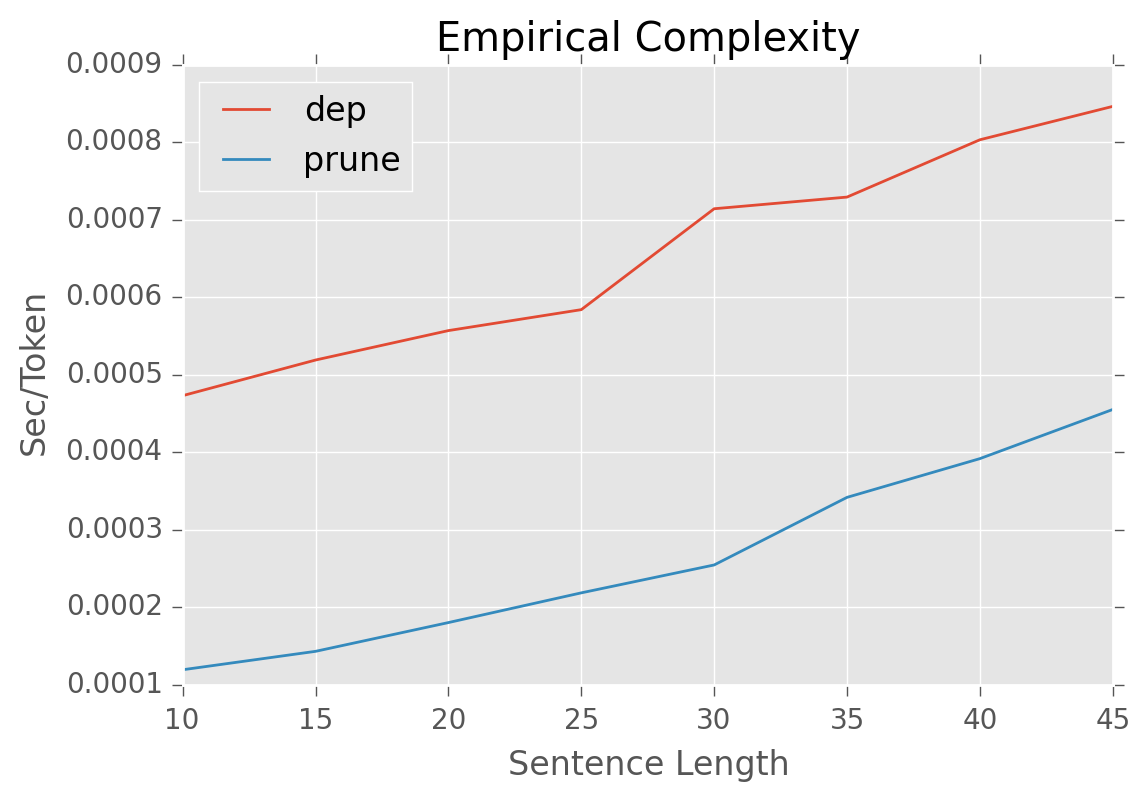
\includegraphics[scale=0.4]{../notebooks/comp}
  \label{tab:speed}
  \caption{Experiments of parsing speed. (a) The speed of the parser on its own and with pruning. (b) The end-to-end speed of the parser when combined with different dependency parsers. }
\end{table}




\section{Conclusion}

With recent advances in statistical dependency parsing, state-of-the-art parsers
have reached the comparable  dependency accuracy as the best phrase structure parsers. However,
these parser cannot be directly used in applications that require phrase-structure prediction. In this work
we have described a simple parsing algorithm and structured prediction system for this comparison, and show that it
can produce phrase-structure parses at comparable accuracy to state-of-the-art system.

One question for future work is whether these results are language
dependent, or whether these transformation can be projected across
languages. If this were possible, we could use a system of this form to learn phrase
structure parsers on languages with only dependency annotations.





% \appendix{}

% \section{Proof of PS Size}
% \label{app:proof}

% Consider the LCFG grammar with two rules $A = \RuleA{X}{X}{X}$ and  $ B = \RuleB{X}{X}{X}$ and a sentence $x_1, \ldots, x_{2n+1}$. Let the dependency parse be defined as $d_{n+1} = 0$ and $d_i = n+1$ for all $i \neq n + 1$, i.e.

% \begin{center}

% \scalebox{0.5}{
% \begin{dependency}[theme=simple]
%   \begin{deptext}[column sep=0.7cm]
%     $1$ \& $2$ \& \ldots \& $n+1$ \& $\ldots$ \& $2n$ \& $2n+1$ \\
%   \end{deptext}
%   \deproot{4}{ROOT}
%   \depedge{4}{1}{}
%   \depedge{4}{2}{}
%   \depedge{4}{6}{}
%   \depedge{4}{7}{}
% \end{dependency}
% }
% \end{center}

% \noindent Since all rules have $h = x_n$ as head, a parse is a chain of $2n$ rules with each rule in $\{A, B\}$, e.g. the following are $BB...$, $BA...$, $AA...$

% \begin{center}

% \scalebox{0.6} {
% \Tree [ .X $x_1$ [ .X $x_2$  [ .$\vdots$ $x_{n+1}$ ]   ] ]
% \Tree [ .X $x_1$ [ .X  [ .$\vdots$ $x_{n+1}$ ] $x_{2n+1}$  ] ]
% \Tree [ .X  [ .X  [ .$\vdots$ $x_{n+1}$ ]   $x_{2n}$ ] $x_{2n+1}$ ]
% }
% \end{center}


% \noindent Since there must be equal $A$s and $B$s and all orders are possible, there are $2n \choose n$ valid parses and $|\mathcal{Y}(x, d)|$ is $O(2^n)$.
% \textbf{Acknowledgment} sections should go as a last (unnumbered) section immediately
% before the references.



\bibliography{full}
\bibliographystyle{naaclhlt2015}

\end{document}

%%% Local Variables:
%%% mode: latex
%%% TeX-master: t
%%% End
